\section{The Adiabatic Approximation II}
\subsection{Analogy with Magnetic Fields}
We found a formula for Berry's Phase last class to be written in terms of an integral over configuration space:
\begin{equation}
    \gamma(T) = i\oint \braket{\psi_n}{\nabla_\v{R}\psi_n} \cdot d\v{R}
\end{equation}
We can rewrite this as:
\begin{equation}
    \gamma = \oint \v{A} \cdot d\v{R}
\end{equation}
where $\v{A} = i\bra{\psi}\nabla_\v{R}\ket{\psi}$. The choice of symbol here is elucidated in the case where we consider a 3-dimensional configurational space, where the Berry's phase formula is reminiscent of the flux from a magnetic field $\v{B}$:
\begin{equation}
    \gamma = \oint \v{A} \cdot d\v{r} = \int_S (\nabla \times \v{A}) \cdot d\v{a} = \int \v{B} \cdot d\v{a}
\end{equation}
where we have used Stoke's theorem to convert from a loop/line integral of $\v{A}$ to a surface integral of the curl of $\v{A}$, and then identified $\v{B} = \nabla \times \v{A}$. Thus, we can consider Berry's phase to be the ``magnetic flux'' resulting from the magnetic field/Berry's curvature $\v{B} = \nabla \times \v{A}$. 

\subsection{Example - Spin-1/2 in B-field}
In the previous section we discussed how the Berry's phase looks like the flux of a ``magnetic field'' $\v{B} = \nabla \times \v{A} = \nabla \times (i\bra{\psi}\nabla_\v{R}\ket{\psi})$. In the case where we actually have a real magnetic field, this analogy makes the calculation of the Berry's phase quite simple. In the previous section we considered the Berry's phase resulting from a magnetic field precessing around the $z$-axis at a fixed angle $\alpha$. Let us now generalize this to the case where the magnetic field sweeps out an arbitrary closed curve on the surface of a sphere of radius $r = B_0$. 

\begin{figure}[htbp]
    \centering
    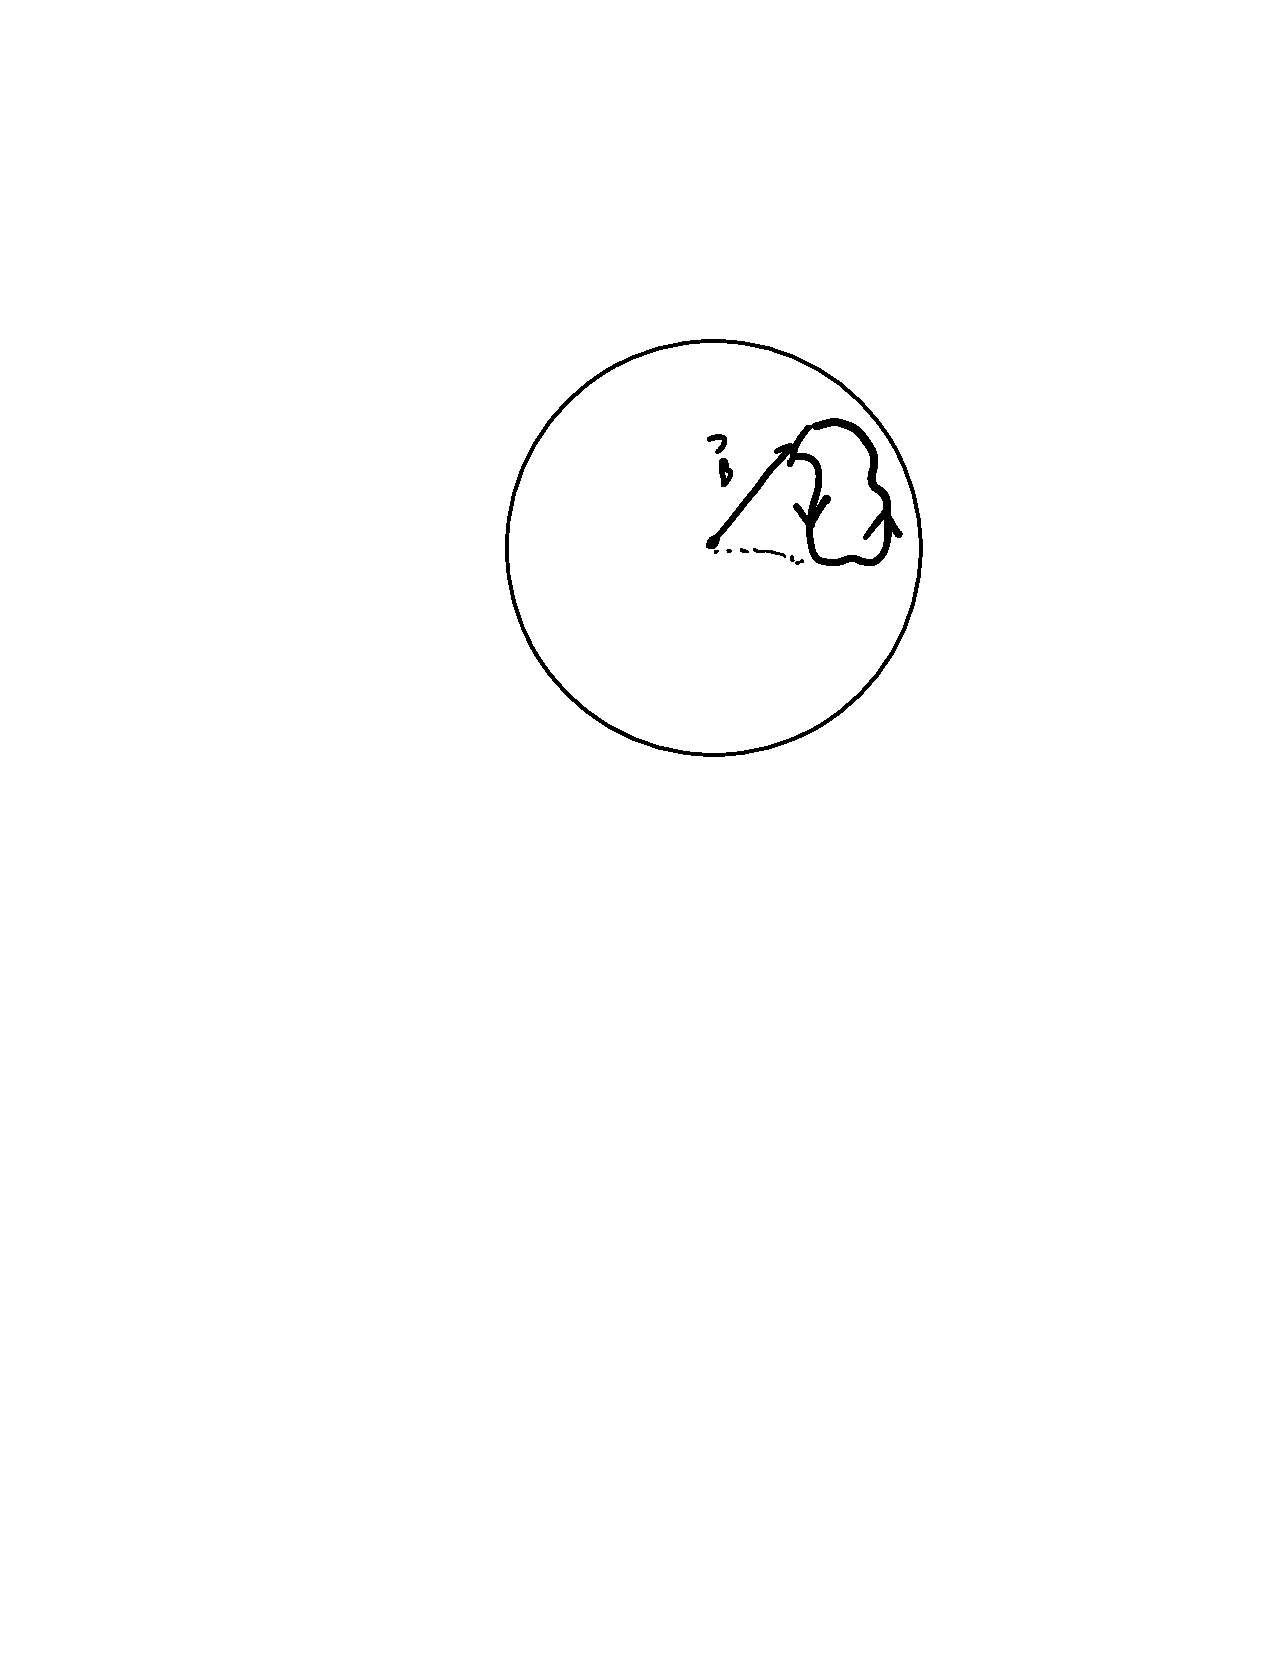
\includegraphics[scale=0.7]{Images/fig-sphereclosedcurve.pdf}

    \caption{We wish to calculate Berry's phase for a magnetic field $\v{B}$ that sweeps out an arbitrary closed curve on a sphere.}
    \label{fig-sphereclosedcurve}
\end{figure}

To this end consider the spinor corresponding to a spin pointing in the direction of $\v{B}(t)$:
\begin{equation}
    \chi_+ = \m{\cos(\frac{\theta(t)}{2}){t} \\ e^{i\phi(t)}\sin(\frac{\theta(t)}{2})}.
\end{equation}
with $\theta(t), \phi(t)$ the polar and azimuthal angles at time $t$. 

We wish to calculate the vector potential $\v{A}$ corresponding to $\v{B}$. To thid end, consider the gradient of $\chi_+$ in polar coordinates:
\begin{equation}
    \nabla \chi_+ = \rhat \dpd{}{r}\chi_+ + \frac{\thetahat}{r}\dpd{}{\theta}\chi_+ + \frac{\phihat}{r\sin\theta}\dpd{}{\phi}\chi_+ = \frac{1}{r}\left[\thetahat\m{-\frac{1}{2}\sin(\frac{\theta}{2}) \\ \frac{1}{2}e^{i\phi}\cos(\frac{\theta}{2})} + \frac{\phihat}{\sin\theta}\m{0 \\ e^{i\phi}\sin(\frac{\theta}{2})}\right]
\end{equation}
and so:
\begin{equation}
    \braket{\chi_+}{\nabla \chi_+} = \frac{1}{r}\thetahat\left[-\frac{1}{2}\sin(\frac{\theta}{2})\cos(\frac{\theta}{2}) + \frac{1}{2}\sin(\frac{\theta}{2})\cos(\frac{\theta}{2})\right] + i\frac{\phihat}{r\sin\theta}\sin^2(\frac{\theta}{2}) = i\frac{\phihat}{r\sin\theta}\sin^2(\frac{\theta}{2})
\end{equation}
and so:
\begin{equation}
    \v{A} = i\braket{\chi_+}{\nabla \chi_+} = -\phihat\frac{\sin^2(\frac{\theta}{2})}{r\sin\theta}
\end{equation}
Therefore recalling the Berry's phase as:
\begin{equation}
    \gamma = \oint \v{A} \cdot d\v{R} = \int \v{B} \cdot d\v{a}
\end{equation}